\documentclass{article}
\usepackage{pgf}
\usepackage{pgfpages}
\usepackage{seqsplit}

\newcommand{\hash}[1]{{\ttfamily\seqsplit{#1}}}

\pgfpagesdeclarelayout{boxed}
{
  \edef\pgfpageoptionborder{0pt}
}
{
  \pgfpagesphysicalpageoptions
  {%
    logical pages=1,%
  }
  \pgfpageslogicalpageoptions{1}
  {
    border code=\pgfsetlinewidth{2pt}\pgfstroke,%
    border shrink=\pgfpageoptionborder,%
    resized width=.95\pgfphysicalwidth,%
    resized height=.95\pgfphysicalheight,%
    center=\pgfpoint{.5\pgfphysicalwidth}{.5\pgfphysicalheight}%
  }%
}

\pgfpagesuselayout{boxed}
\usepackage{listings}
\usepackage{xcolor}

\definecolor{codegreen}{rgb}{0,0.6,0}
\definecolor{codegray}{rgb}{0.5,0.5,0.5}
\definecolor{codepurple}{rgb}{0.58,0,0.82}
\definecolor{backcolour}{rgb}{0.95,0.95,0.92}

\lstdefinestyle{mystyle}{
    backgroundcolor=\color{backcolour},   
    commentstyle=\color{codegreen},
    keywordstyle=\color{magenta},
    numberstyle=\tiny\color{codegray},
    stringstyle=\color{codepurple},
    basicstyle=\ttfamily\footnotesize,
    breakatwhitespace=false,         
    breaklines=true,                 
    captionpos=b,                    
    keepspaces=true,                 
    numbers=left,                    
    numbersep=5pt,                  
    showspaces=false,                
    showstringspaces=false,
    showtabs=false,                  
    tabsize=2
}

\lstset{style=mystyle}



\usepackage[top=3cm, bottom=4cm, left=3.5cm, right=3.5cm]{geometry}
\usepackage{amsmath,amsthm,amsfonts,amssymb,amscd, fancyhdr, color, comment, graphicx, environ}
\usepackage{float}
\usepackage{mathrsfs}
\usepackage[math-style=ISO]{unicode-math}
\setmathfont{TeX Gyre Termes Math}
\usepackage{lastpage}
\usepackage[dvipsnames]{xcolor}
\usepackage[framemethod=TikZ]{mdframed}
\usepackage[shortlabels]{enumitem}
\usepackage{fancyhdr}
\usepackage{indentfirst}
\usepackage{listings}
\usepackage{sectsty}
\usepackage{thmtools}
\usepackage{shadethm}
\usepackage{hyperref}
\usepackage{setspace}
\hypersetup{
    colorlinks=true,
    linkcolor=blue,
    filecolor=magenta,      
    urlcolor=blue,
}

\mdfsetup{skipabove=\topskip,skipbelow=\topskip}
\newrobustcmd\ExampleText{%
An \textit{inhomogeneous linear} differential equation has the form
\begin{align}
L[v ] = f,
\end{align}
where $L$ is a linear differential operator, $v$ is the dependent
variable, and $f$ is a given non−zero function of the independent
variables alone.
}
\mdfdefinestyle{theoremstyle}{%
linecolor=black,linewidth=1pt,%
frametitlerule=true,%
frametitlebackgroundcolor=gray!20,
innertopmargin=\topskip,
}
\mdtheorem[style=theoremstyle]{Problem}{Problem}
\newenvironment{Solution}{\textbf{Solution.}}


\newcommand{\norm}[1]{\left\lVert#1\right\rVert}     
\newcommand\course{Course}                        
\newcommand\hwnumber{2}                              
\newcommand\Information{XXX/xxxxxxxx}       
\pagestyle{}
\pagenumbering{arabic}
\cfoot{\small\thepage}

\renewcommand{\labelenumi}{\alph{enumi})}
\newcommand{\Z}{\mathbb Z}
\newcommand{\R}{\mathbb R}
\newcommand{\Q}{\mathbb Q}
\newcommand{\NN}{\mathbb N}
\DeclareMathOperator{\Mod}{Mod} 
\renewcommand\lstlistingname{Algorithm}
\renewcommand\lstlistlistingname{Algorithms}
\def\lstlistingautorefname{Alg.}




\begin{document}

\begin{titlepage}
    \begin{center}
        \vspace*{3cm}
            
        \Huge
        \textbf{Homework 4}
            
        \vspace{1cm}
        \huge
        
            
        \vspace{1.5cm}
      \huge
            
        \centering
        \textbf{Priyanka Emani - 1001981861} 
        \centering
        \newline
        \textbf{Aravind Kashyap - 1001956591}
        \centering
        \newline
        \textbf{Shreyas Jagadeep - 1001888859}
        
            
       
        \vspace{1cm}
            \begin{figure}[h!]
                \centering
                
\includegraphics[width=0.75\textwidth]{1280px-University_of_Texas_at_Arlington_logo.svg.png}
                        \label{fig:my_label}
            \end{figure}
       
        \vspace{2cm}
        \huge
       \textbf{CSE: 5370 Bioinformatics} 
            
        \\
      
  \huge
        \vspace{2cm}
       \huge
        
        \today
            
    \end{center}
\end{titlepage}
\newpage

\section*{Collaboration Statement}
The assignment was carried out as a group. Following students were part of the group and made
individual contributions in completing the assignment.


\newpage

\section*{ 1. Bioinformatics}

\begin{question}
    
Single Cell RNA Analysis. The dataset used describes single-cell mouse tissues. The dataset
contains 100,000 cells from the brain of a mouse. Each column in the expression matrix csv file
corresponds to a a transcript (gene) wherelese each row corresponds to a single cell. The metadata
csv file describes each cell.

\end{question}
    
\section*{2. Imports and Data Objects}
   

\begin{lstlisting}[language=Python]
from sklearn.cluster import KMeans
import matplotlib.pyplot as plt
import scanpy as sc
import pandas as pd
import numpy as np
%matplotlib inline

count = pd.read_csv('/content/drive/MyDrive/data/brain_counts.csv', index_col=0)
metadata = pd.read_csv('/content/drive/MyDrive/data/brain_metadata.
,→csv',index_col=0)
adata = sc.AnnData(X = count, obs = metadata)

\end{lstlisting}

\section*{3. Preprocessing}

1.0 Spiked genes
\begin{lstlisting}[language=Python]
# record and keep count of spikes
is_spiked = {}
num_spikes = 0
for gene in adata.var_names:
if 'ERCC' in gene:
is_spiked[gene] = True
num_spikes += 1
else:
is_spiked[gene] = False
adata.var['ERCC'] = pd.Series(is_spiked)
# write
adata.write('/content/drive/MyDrive/data/brain_raw.h5ad')
# read
adata = sc.read('/content/drive/MyDrive/data/brain_raw.h5ad')
\end{lstlisting}

2.0 Quality control
\begin{lstlisting}[language=Python]
# Compute QC Metrics
qc = sc.pp.calculate_qc_metrics(adata, qc_vars = ['ERCC'])
cell_qc = qc[0]
gene_qc = qc[1]

\end{lstlisting}
 qc - cells

\begin{lstlisting}[language=Python]


# visualize spike-ins
# outliers to be filtered
plt.hist(cell_qc['pct_counts_ERCC'], bins=1000)
plt.xlabel('Percentage Count (ERCC)')
plt.ylabel('Number of Cells')
plt.axvline(10, color='red')
\end{lstlisting}
<matplotlib.lines.Line2D at 0x7fdffb780c50>

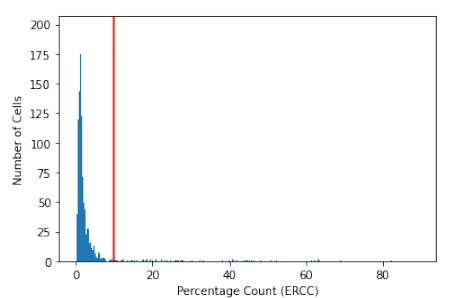
\includegraphics[]{Table-1.png}

\begin{lstlisting}[language=Python]
# visualize lib size (reads per cell)
# cell with few reads to be filtered
plt.hist(cell_qc['total_counts'], bins=1000)
plt.xlabel('Count')
plt.ylabel('Number of Cells')
plt.axvline(50000, color='red')
\end{lstlisting}
<matplotlib.lines.Line2D at 0x7fdffad67710>

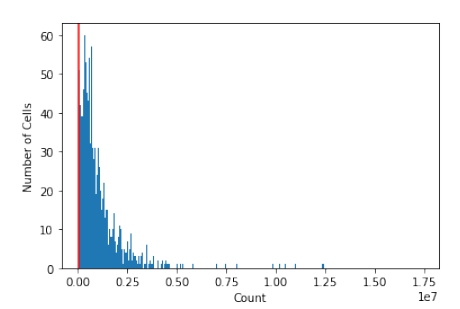
\includegraphics[]{Table-2.png}

\begin{lstlisting}[language=python]
# visualize detected gene-count (in cells)
# outliers to be filtered
plt.hist(cell_qc['n_genes_by_counts'], bins=100)
plt.xlabel('Number of Genes')
plt.ylabel('Number of Cells')
plt.axvline(1000, color='red')
\end{lstlisting}
<matplotlib.lines.Line2D at 0x7fdffa2f8150>


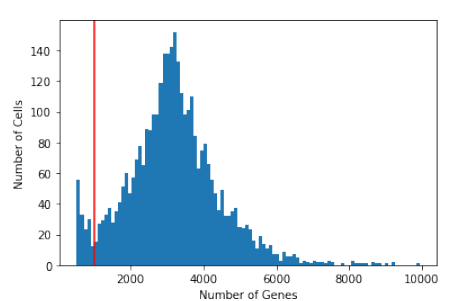
\includegraphics[]{Table-3.png}
\begin{lstlisting}[language=Python]
# filtering
# by ERCC
low_ERCC = (cell_qc['pct_counts_ERCC'] < 10)
adata = adata[low_ERCC]
# by Gene count
sc.pp.filter_cells(adata, min_genes = 1000)
# write
adata.write('/content/drive/MyDrive/data/brain_qc.h5ad')
# read
adata = sc.read('/content/drive/MyDrive/data/brain_qc.h5ad')
\end{lstlisting}

\newline 3.0 Normalization
\newline Cell library normalization
\begin{lstlisting}[language=python]

# visualization of data before Normalization
sc.pp.pca(adata)
sc.pl.pca_overview(adata, color='mouse.id')
\end{lstlisting}

\begin{figure}
    \centering
    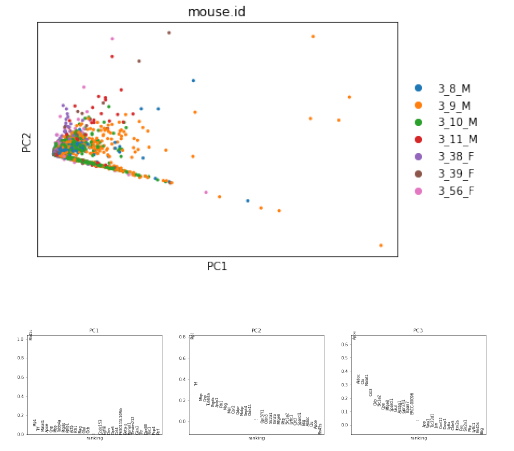
\includegraphics{4.png}
  \end{figure}
  \begin{figure}
    \centering
    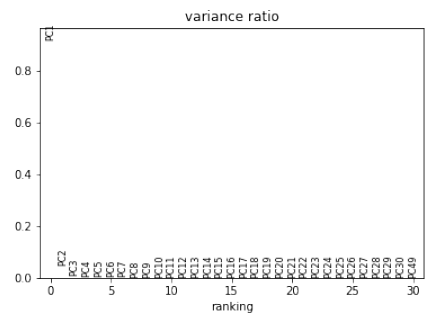
\includegraphics{5.png}
  \end{figure}
  \newpage
  \begin{lstlisting}[language=python]
  # copy data. copy and original to be used for comparison
adata_ = adata.copy()
# copy data before normalizing
adata_.raw = adata_
# CPM normalization
sc.pp.normalize_per_cell(adata_,counts_per_cell_after=1e6)
# visualization of data after Normalization
sc.pp.pca(adata_)
sc.pl.pca_overview(adata_, color='mouse.id')
  \end{lstlisting}
  
  \begin{figure}
      \centering
      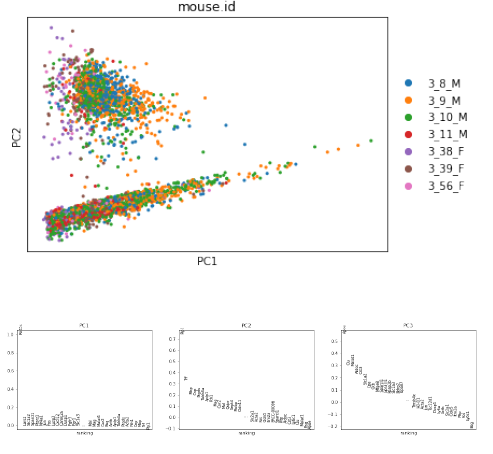
\includegraphics{6.png}
        \end{figure}
        \begin{figure}
      \centering
      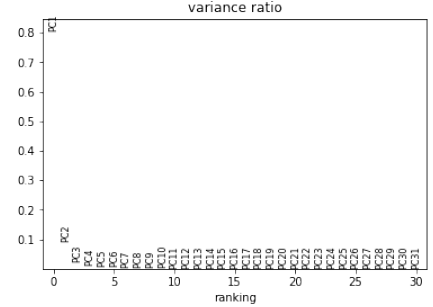
\includegraphics{7.png}
        \end{figure}
        \newpage
    Gene expression normalization
    
    \begin{lstlisting}[language=python]
# Rn45s gene is dorminant in data.
# Use normalization to deal with imbalance
Rn45s_0 = adata_.var.index != 'Rn45s'
adata_Rn45s_0 = adata_[:, Rn45s_0]
# visualization of data after Normalization
sc.pp.pca(adata_Rn45s_0)
sc.pl.pca_overview(adata_Rn45s_0, color='mouse.id')
    \end{lstlisting}
    
\begin{figure}
      \centering
      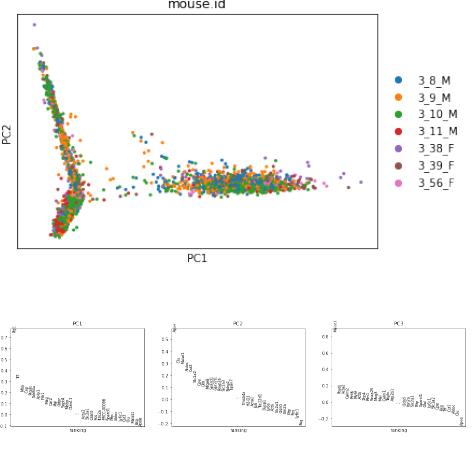
\includegraphics{8.png}
        \end{figure}
\begin{figure}
      \centering
      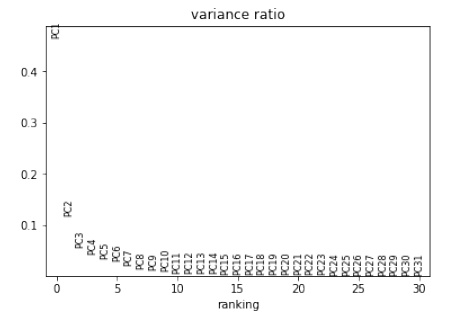
\includegraphics{9.png}
        \end{figure}
\begin{lstlisting}[language=python]
        # centering and scaling gene expression data
sc.pp.log1p(adata_)
sc.pp.scale(adata_)
# visualization after Normalization
sc.pp.pca(adata_)
sc.pl.pca_overview(adata_, color='plate.barcode')
\end{lstlisting}
\begin{figure}
    \centering
    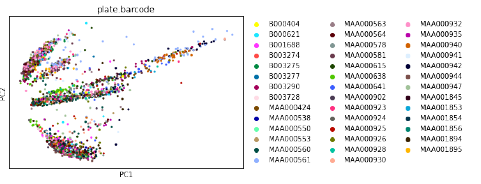
\includegraphics{10.png}
\end{figure}        
\begin{figure}
    \centering
    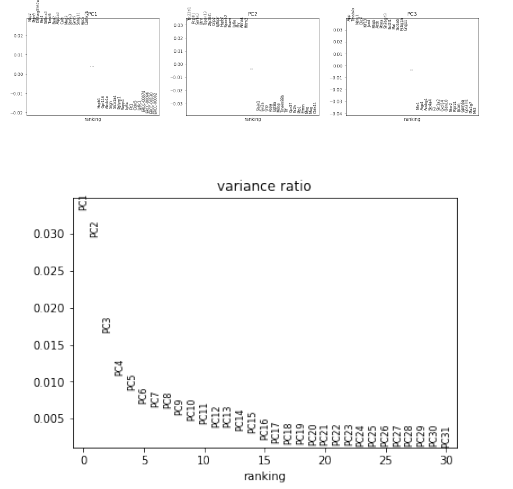
\includegraphics{11.png}
\end{figure}         
\begin{lstlisting}[language=python]
# write
adata_.write('/content/drive/MyDrive/data/brain_normalized.h5ad')
# read
adata = sc.read('/content/drive/MyDrive/data/brain_normalized.h5ad')
\end{lstlisting}

\section*{4. Analysis}

Dimensionality Reduction -UMAP

\begin{lstlisting}[language=Python]
sc.pp.neighbors(adata)
sc.tl.umap(adata, min_dist=0.5, spread=1.0, n_components=2)
# UMAP visualization using Dimensionality Reduction
sc.pl.umap(adata, color='cell_ontology_class')
\end{lstlisting}

\begin{figure}
    \centering
    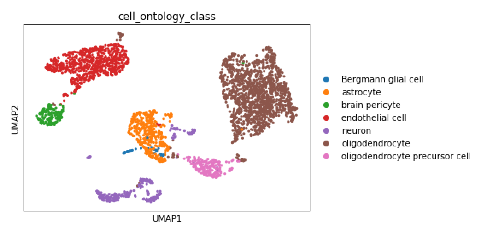
\includegraphics{12.png}
\end{figure}
Clustering - UMAP
\begin{lstlisting}[language=Python]

umap_= adata.obsm['X_umap']
kmeans = KMeans(n_clusters=4).fit(umap_)
adata.obs['K Means Clustering'] = kmeans.labels_
adata.obs['K Means Clustering'] = adata.obs['K Means Clustering'].astype(str)
# UMAP visualization using KMeans Clsutering
sc.pl.umap(adata, color='K Means Clustering')
\end{lstlisting}
        
\begin{figure}
    \centering
    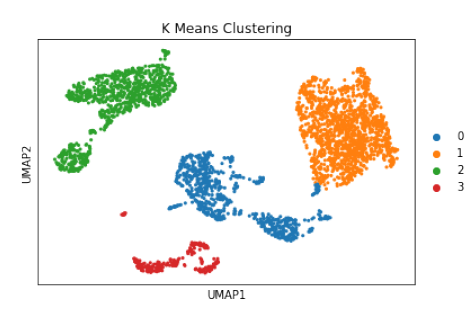
\includegraphics{13.png}
\end{figure}        

\newpage
\section*{References}
Below are the list of references we used for this project.
\newline
1. https://github.com/scverse/scanpy-tutorials/issues/28
\newline
2. https://www.ncbi.nlm.nih.gov/geo/query/acc.cgi?acc=GSM3109048
\newline
3. https://www.ncbi.nlm.nih.gov/geo/query/acc.cgi?acc=GSE49712
\newline
4. https://scanpy.readthedocs.io/en/stable/generated/scanpy.pp.calculate_qc_metrics.html
\newline
5. https://github.com/scverse/scanpy/issues/978
\newline
6. https://github.com/scverse/scanpy/issues/1147
\newline7. https://www.oreilly.com/library/view/python-data-science/9781491912126/ch04.html
\newline
8. https://matplotlib.org/stable/tutorials/introductory/pyplot.html
\newline
9. https://chanzuckerberg.github.io/scRNA-python-workshop/preprocessing/01-basic-qc.html
\newline
10. https://github.com/AmoDinho/datacamp-python-data-science-track/blob/master/Machine%20Learning%20with%20Experts-School%20Budgets/Chapter%201%20-%20Exploring%20the%20raw%20data.py
\newline
11. https://scanpy.readthedocs.io/en/stable/generated/scanpy.pp.filter_cells.html
\newline
12. https://scanpy.readthedocs.io/en/stable/generated/scanpy.pl.pca.html
\newline
13. https://github.com/scverse/scanpy/issues/324
\newline
14. https://nbisweden.github.io/workshop-scRNAseq/labs/compiled/scanpy/scanpy_04_clustering.html
\newline
15. https://scanpy.readthedocs.io/en/stable/generated/scanpy.pp.normalize_per_cell.html
\newline
16. https://scanpy.readthedocs.io/en/stable/generated/scanpy.pp.normalize_total.html
\newline
17. https://www.ncbi.nlm.nih.gov/pmc/articles/PMC4404308/
\newline
18. https://scanpy.readthedocs.io/en/stable/generated/scanpy.tl.umap.html
\newline
19. https://scanpy.readthedocs.io/en/stable/generated/scanpy.pp.neighbors.html
\newline
20. https://github.com/scverse/scanpy/blob/master/scanpy/tools/_umap.py
\newline
21. https://github.com/theislab/scvelo/issues/37
\newline
22. https://towardsdatascience.com/umap-and-k-means-to-classify-characters-league-of-legends-668a788cb3c1
\newline
23. https://umap-learn.readthedocs.io/en/latest/clustering.html
\newline
24. https://scanpy.readthedocs.io/en/stable/generated/scanpy.pp.log1p.html

\newline
Also we have taken help from Dr. Steven Fernandes who is post doctoral research at University of Central Florida


\end{document}

